\documentclass{ZenTera}
\runningheader{EA722}{Experimento 2}{\today}
\footer{}{\thepage}{}

\title{\textbf{EA722 --- Laboratório de Controle e Servomecanismo\vspace{7mm}\\\large Experimento 2 --- Fundamentos de Realimentacão: Controle em Malha Aberta e Fechada (Proporcional) dos Sistemas ECPs} }

\author{Lucas Guimarães Braga \\RA: 182543 \and Lucas Zenichi Terada \\RA: 182775 \and Nícolas F. R. A. Prado \\RA: 185142}
\date{\today}

\begin{document}
%    \begin{figure}
        \begin{minipage}{.5\linewidth}
            \flushleft
            
\includegraphics[height=1in]{0_img/logo_unicamp.jpg}
        \end{minipage}%
        \begin{minipage}{.5\linewidth}
            \flushright
            
\includegraphics[width=1.4in]{0_img/logo_feec.png}
        \end{minipage}
    \end{figure}
\maketitle 


Observações em aula:

\textbf{item 4:} 
\begin{itemize}
    \item Presença de não linearidades e imperfeições no sistema que deformam o gráfico e causam o erro em regime;

    \item Observação: O erro em regime é visto na entrada diferente de zero;
    
    \item mudança do $k_{pf}$ para o valor de 0.0330 utilizando um método de proporção, mas ainda sim o valor não chegou em regime.
    
    \item Mudança do $k_{pf}$ para o valor de 0.0302
    
    \item Mudança do $k_{pf}$ para o valor de 0.02785
\end{itemize}

\textbf{item 6:}
\begin{itemize}
    \item $K_p = [0.03, 0.12, 0.24]$ e $K_{pf} = [2.5839, 1.3960, 1.1980] $. Novos valores de $k_{pf} = [1.9900,1.2449,1.11997]$
\end{itemize}

\textbf{Item 7:}
\begin{itemize}
    \item Para malha fechada:
    
    \item Para malha aberta:
\end{itemize}

\begin{questions}
\question Mostre os resultados obtidos para o sistema em malha aberta e malha fechada, discutindo sobre o problema do erro em regime permanente em ambos os casos.

    \begin{solution}
        Através da planta disponível no laboratório LE31 da FEEC, realizou-se o controle de malha aberta, cujos resultados podem ser vistos nas figuras~\ref{fig:aberta} e \ref{fig:aberta_mola}. 
        Para os resultados do gráfico~\ref{fig:aberta_corrigida}, foi preciso reajustar o valor de $k_{pf}$ para 0.02785 de modo a minimizar o erro em regime, uma vez que o valor teórico não apresentou o resultado esperado como mostra a figura~\ref{fig:aberta}. 
        Utilizando o valor corrigido adicionou-se uma nova mola no sistema, obtendo assim, a figura~\ref{fig:aberta_mola} que, conforme discutido anteriormente no roteiro 1, apresentou um erro em regime.
        
        Da mesma forma que para o sistema de malha aberta, houve a necessidade de ajustar os valores de $k_{pf}$ (para 1.9900, 1.2449 e 1.11997) de modo a minimizar os erros em regime, uma vez que os valores teóricos não foram capazes de anulá-los, como mostra a figura~\ref{fig:fechada}.
        Utilizando os novos valores de $k_{pf}$ para os diferentes $k_p$ do sistema, obteve-se a figura~\ref{fig:fechada_corrigida}.
        Alterando a mola, observa-se a presença de um erro em regime que diminui com o aumento de $k_p$ dado um valor de $k_{pf}$ projetado para anular o erro em regime para a mola anterior.
        
        Obs: era esperado que não houvesse a necessidade de alterar os valores de $k_{pf}$ para a malha fechada e que ela apresentasse um erro em regime muito próximo de zero para o caso em que não é feita a alteração do valor de $k_1$.
        Como foi discutido com o professor em sala de aula, isto pode ter ocorrido por efeitos de não linearidade do sistema.
        Apesar deste efeito, foi possível notar que a sensibilidade para distúrbios (alteração do valor de $k_1$) para o sistema em malha fechada é menor do que o sistema em malha aberta, ou seja, observou-se um erro em regime menor para a malha fechada. 
    \end{solution}

\question Explique o que ocorre com o comportamento do sistema quando o ganho proporcional $k_p$ é progressivamente aumentado, notando de que forma o comportamento regulador do sistema em resposta a um distúrbio é afetado pelo aumento do ganho de malha produzido pelo ganho proporcional.
Apresente os gráficos obtidos a partir dos experimentos para o sistema em malha fechada com diferentes valores de $k_p$.

    \begin{solution}
    Analisando-se os gráficos da figura~\ref{fig:fechada_corrigida}, fica evidente que o aumento do ganho proporcional $k_p$ diminui o tempo de subida do sinal, no entanto, também aumenta o sobre-sinal, número de oscilações e tempo de assentamento. E com a figura~\ref{fig:fechada_mola} é observado o mesmo efeito, porém com erros em regime, que podem ser reduzidos com o aumento de $k_p$, ou seja, o aumento do valor de $k_p$ diminui a influencia dos distúrbios no sistema. 
    \end{solution}
    
\question Explique por que, eventualmente, é necessário ajustar o valor do ganho do pré-filtro na experiência com o sistema operando em malha aberta. 
Mostre um gráfico da resposta ao degrau do sistema (em malha aberta) quando foi utilizado o ganho do pré-filtro obtido teoricamente na experiência 1 e com o valor ajustado empiricamente durante a experiência 2.

    \begin{solution}
    Analisando as figuras~\ref{fig:aberta} e \ref{fig:aberta_corrigida}, pode-se observar que é necessário ajustar o valor de $k_{pf}$ para o sistema em malha aberta, pois o mesmo é muito mais sensível a distúrbios, e se tratando das condições do experimento que não são ideais, uma variação no valor de $k_1$ gera um erro em regime muito maior para o caso de malha aberta do que para o sistema em malha fechada.
    Observando a figura~\ref{fig:aberta} no intervalo $1.5<t<3$ é possível notar claramente o erro em regime causado pelas não linearidades do sistema, que o afeta em malha aberta e fechada, sendo um efeito com mais influência para a malha aberta. 
    
    
    
    \end{solution}

\end{questions}

\appendix

\section{Gráficos}
\begin{figure}[H]
    \centering
    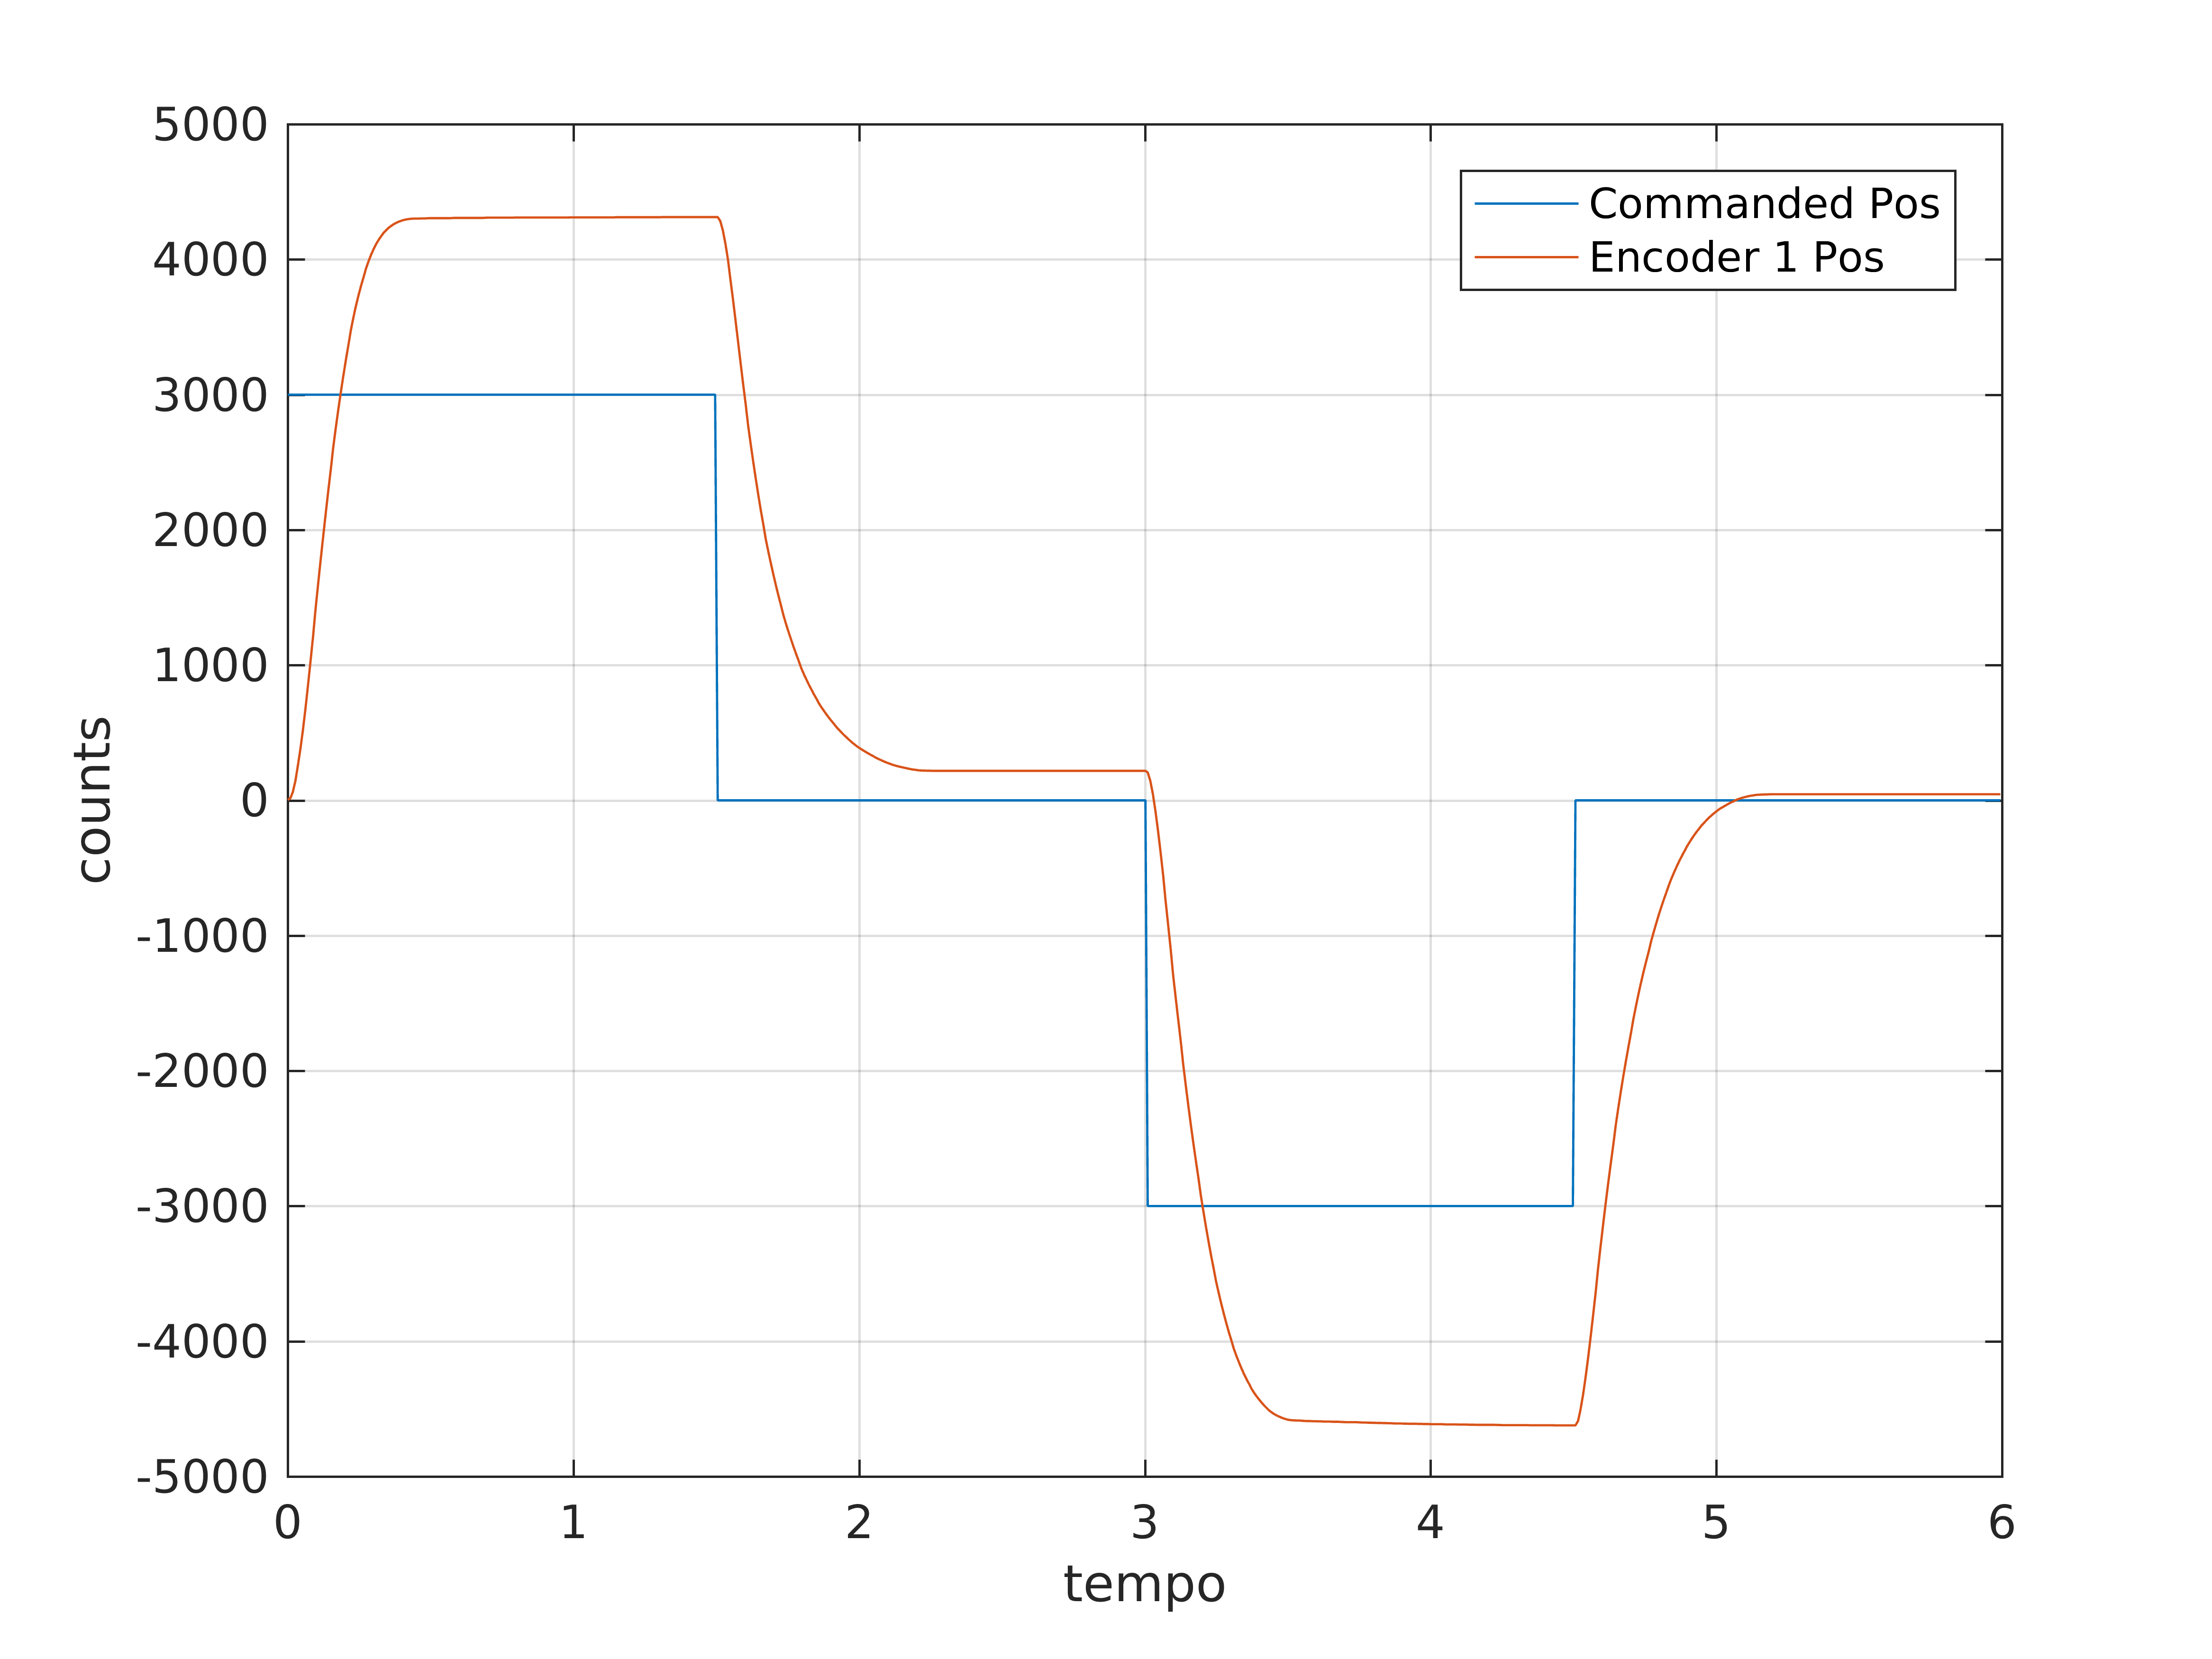
\includegraphics[width=.9\textwidth]{0_img/malha_aberta.png}
    \caption{Saída do sistema em malha aberta com ganho $k_{pf}$ calculado teoricamente para minimizar o erro em regime}
    \label{fig:aberta}
\end{figure}
\begin{figure}
    \centering
    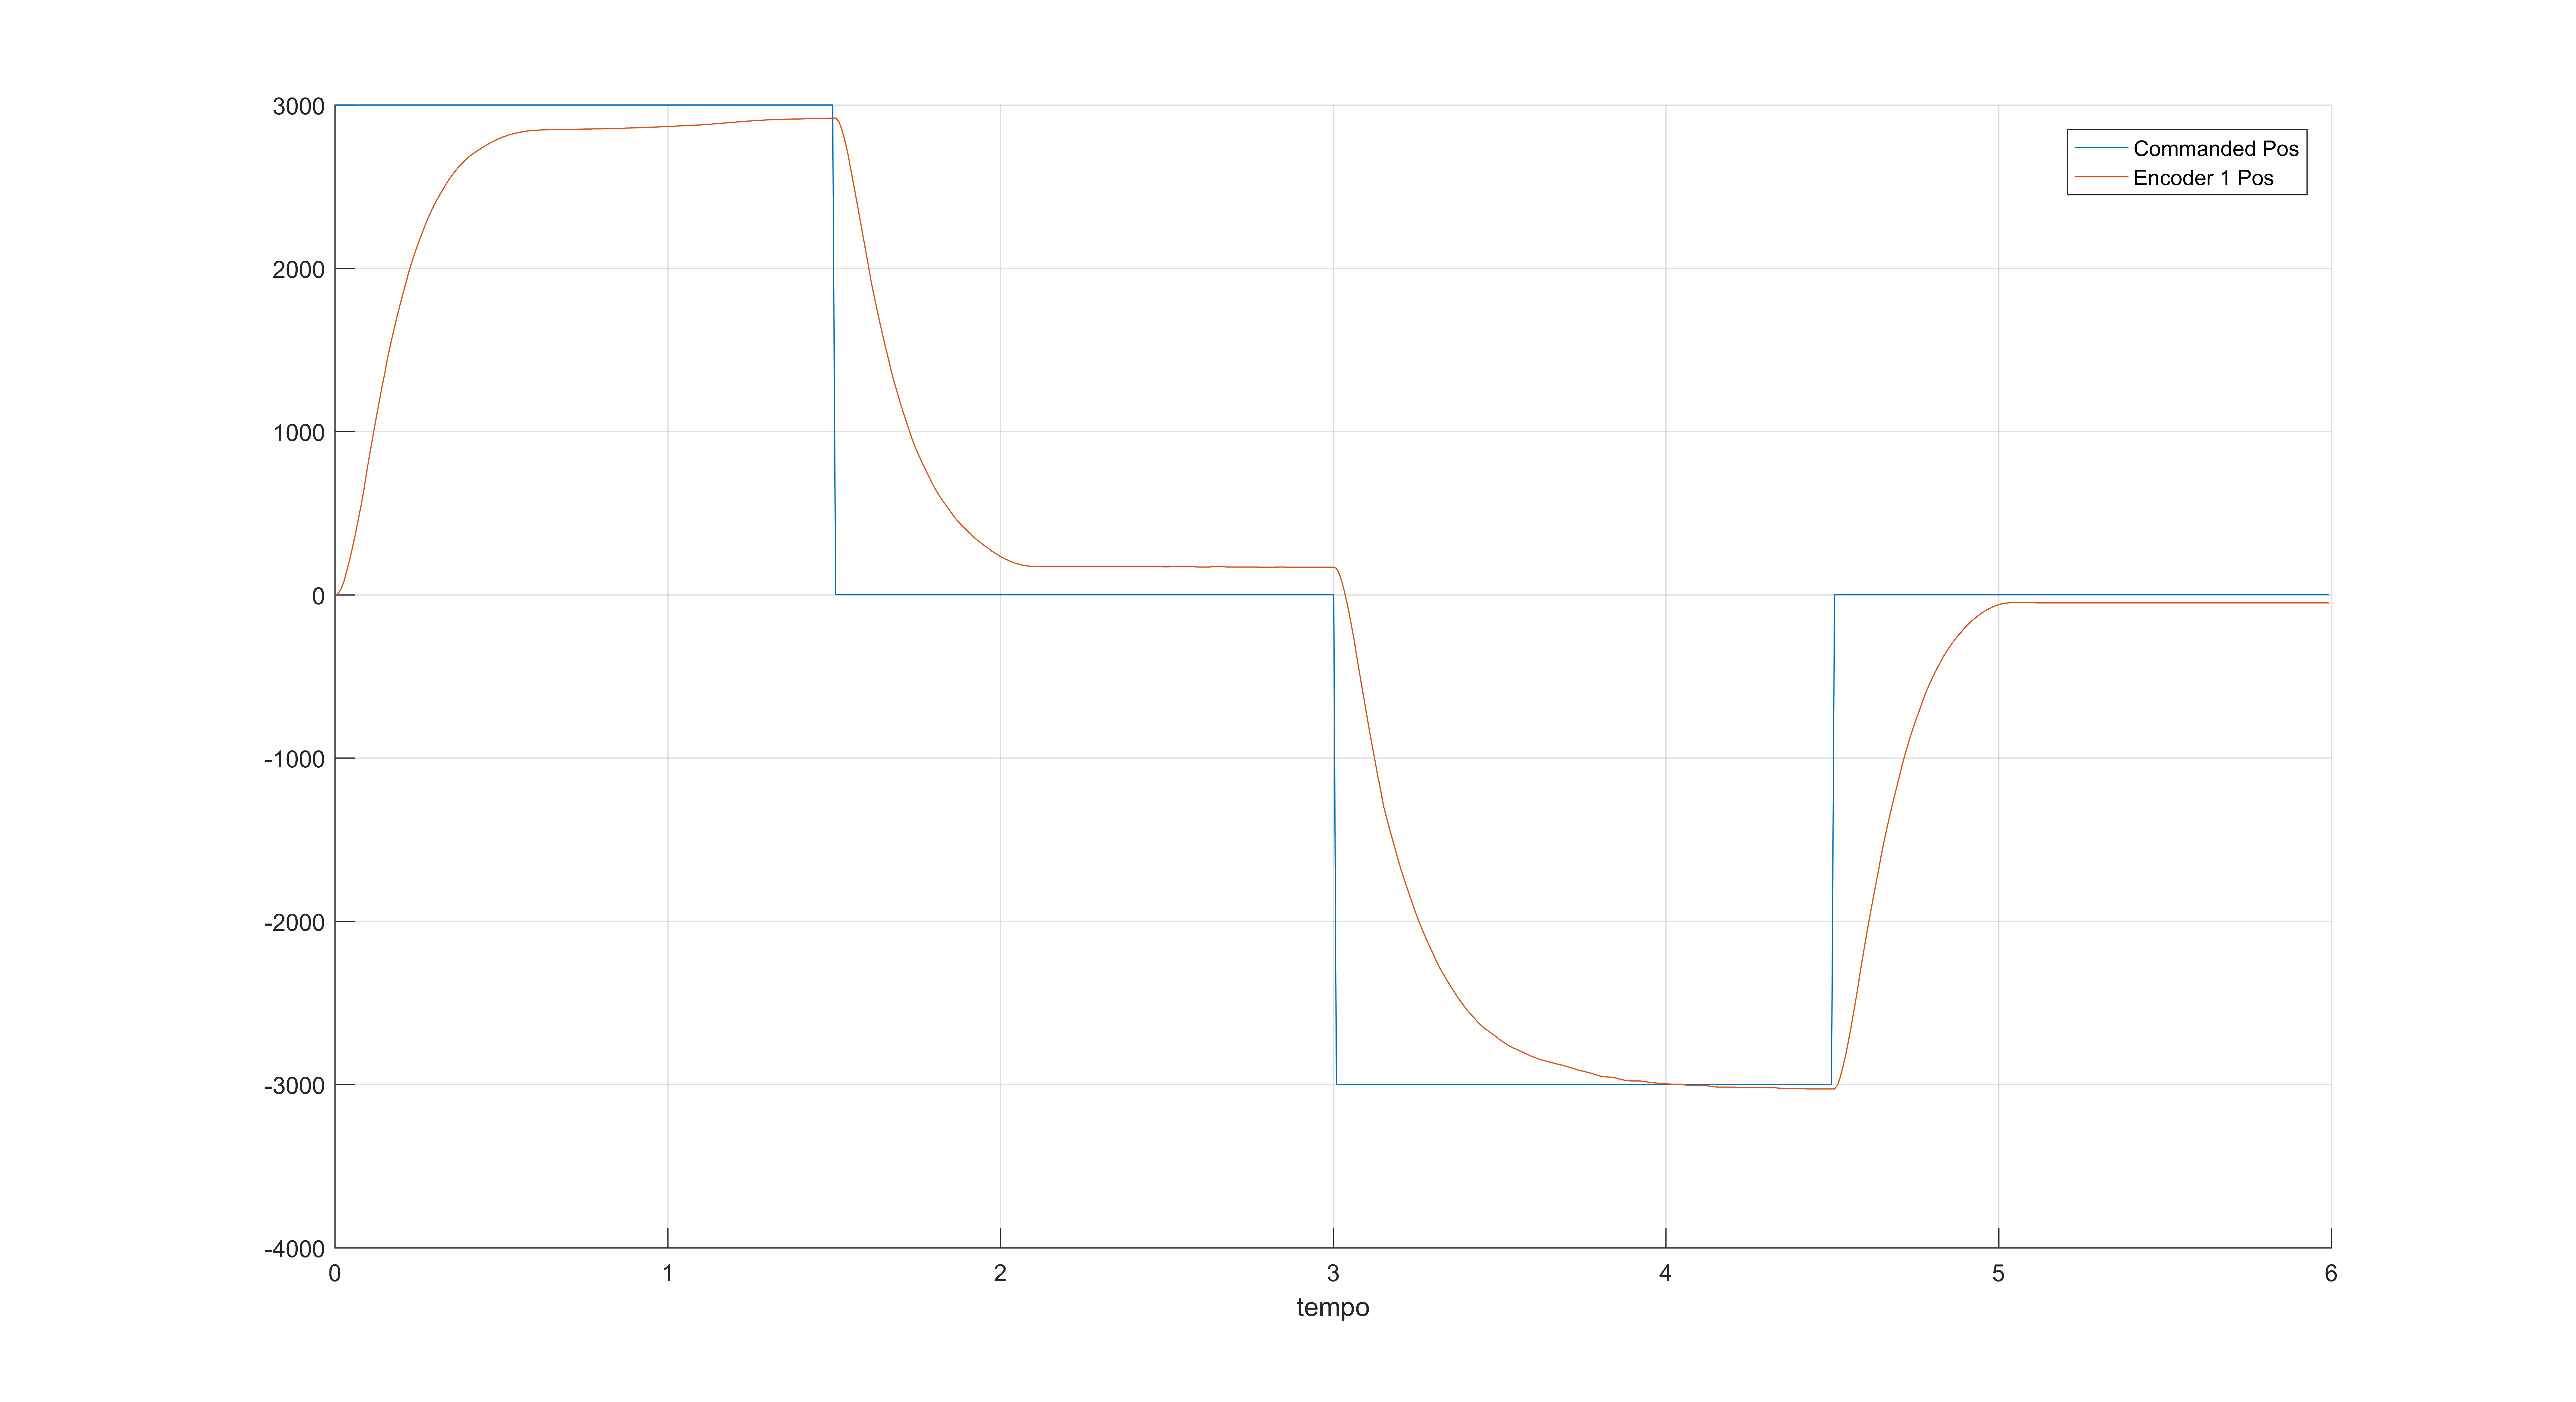
\includegraphics[width=\textwidth]{0_img/malha_aberta_corrigida.png}
    \caption{Saída do sistema em malha aberta com ganho $k_{pf}$ ajustado empiricamente para minimizar o erro em regime}
    \label{fig:aberta_corrigida}
\end{figure}

\begin{figure}
    \centering
    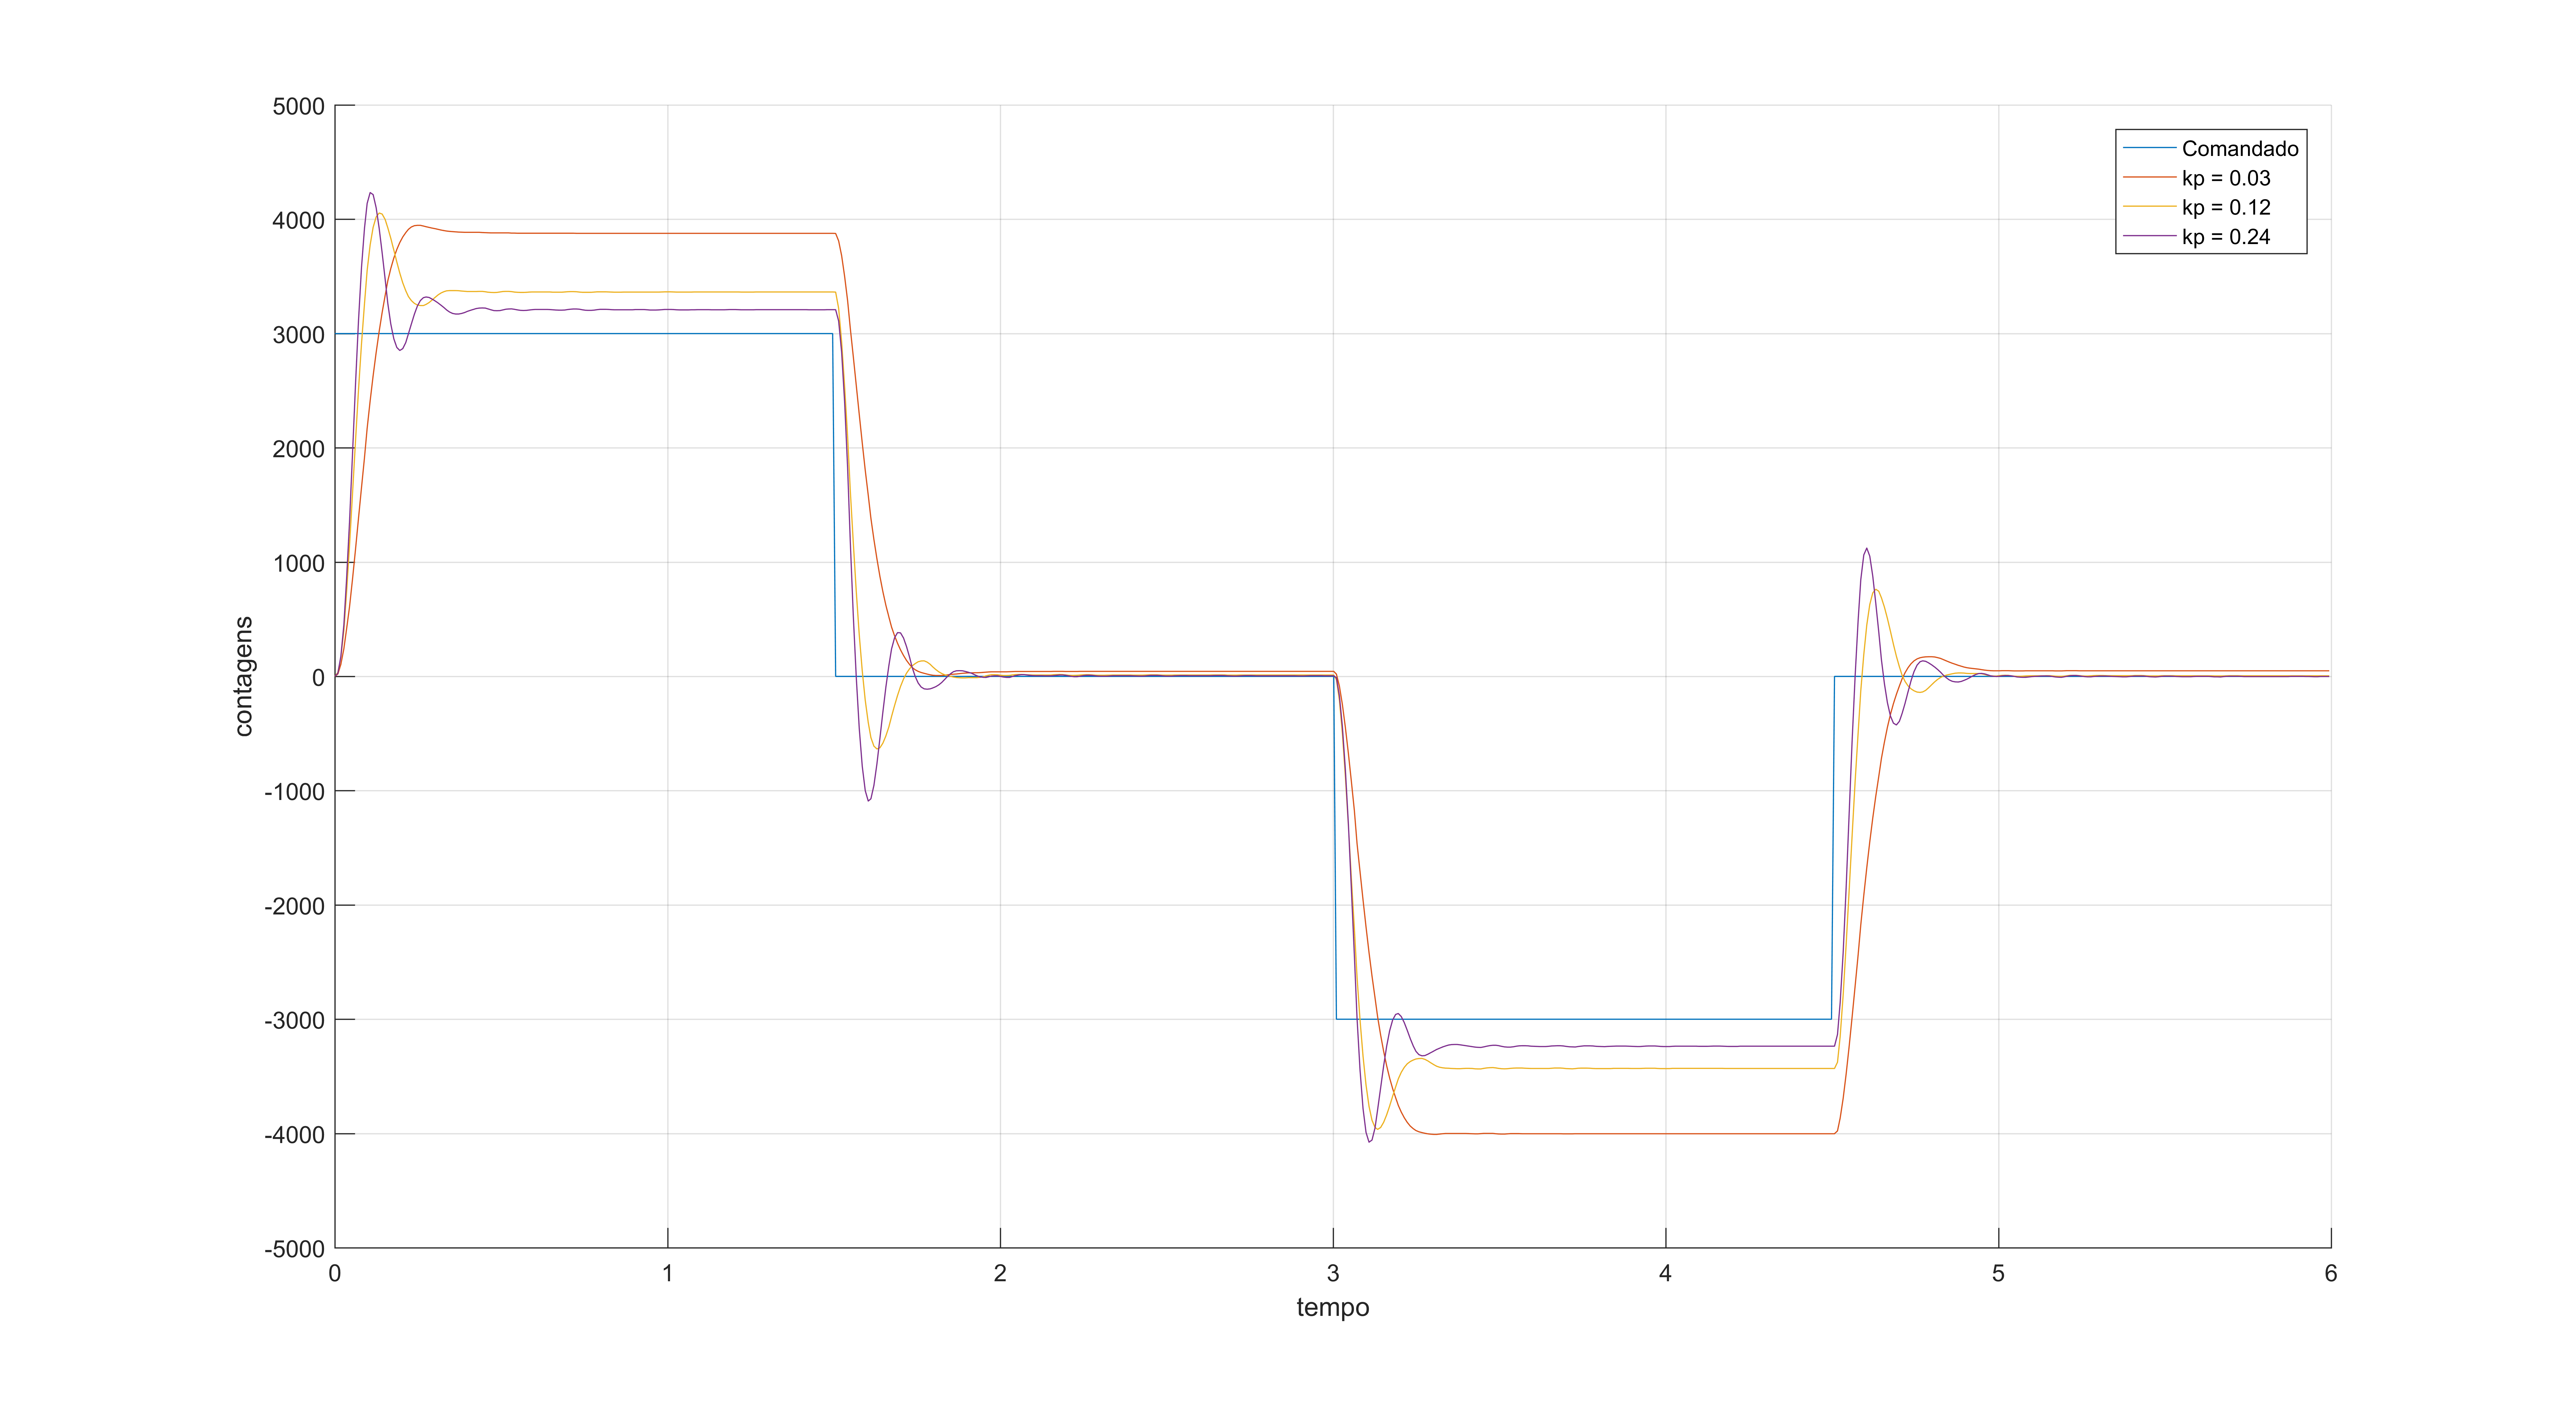
\includegraphics[width=\textwidth]{0_img/malha_fechada.png}
    \caption{Saída do sistema em malha fechada com ganho $k_{pf}$ calculado teoricamente para minimizar o erro em regime e diferentes valores de $k_p$}
    \label{fig:fechada}
\end{figure}
\begin{figure}
    \centering
    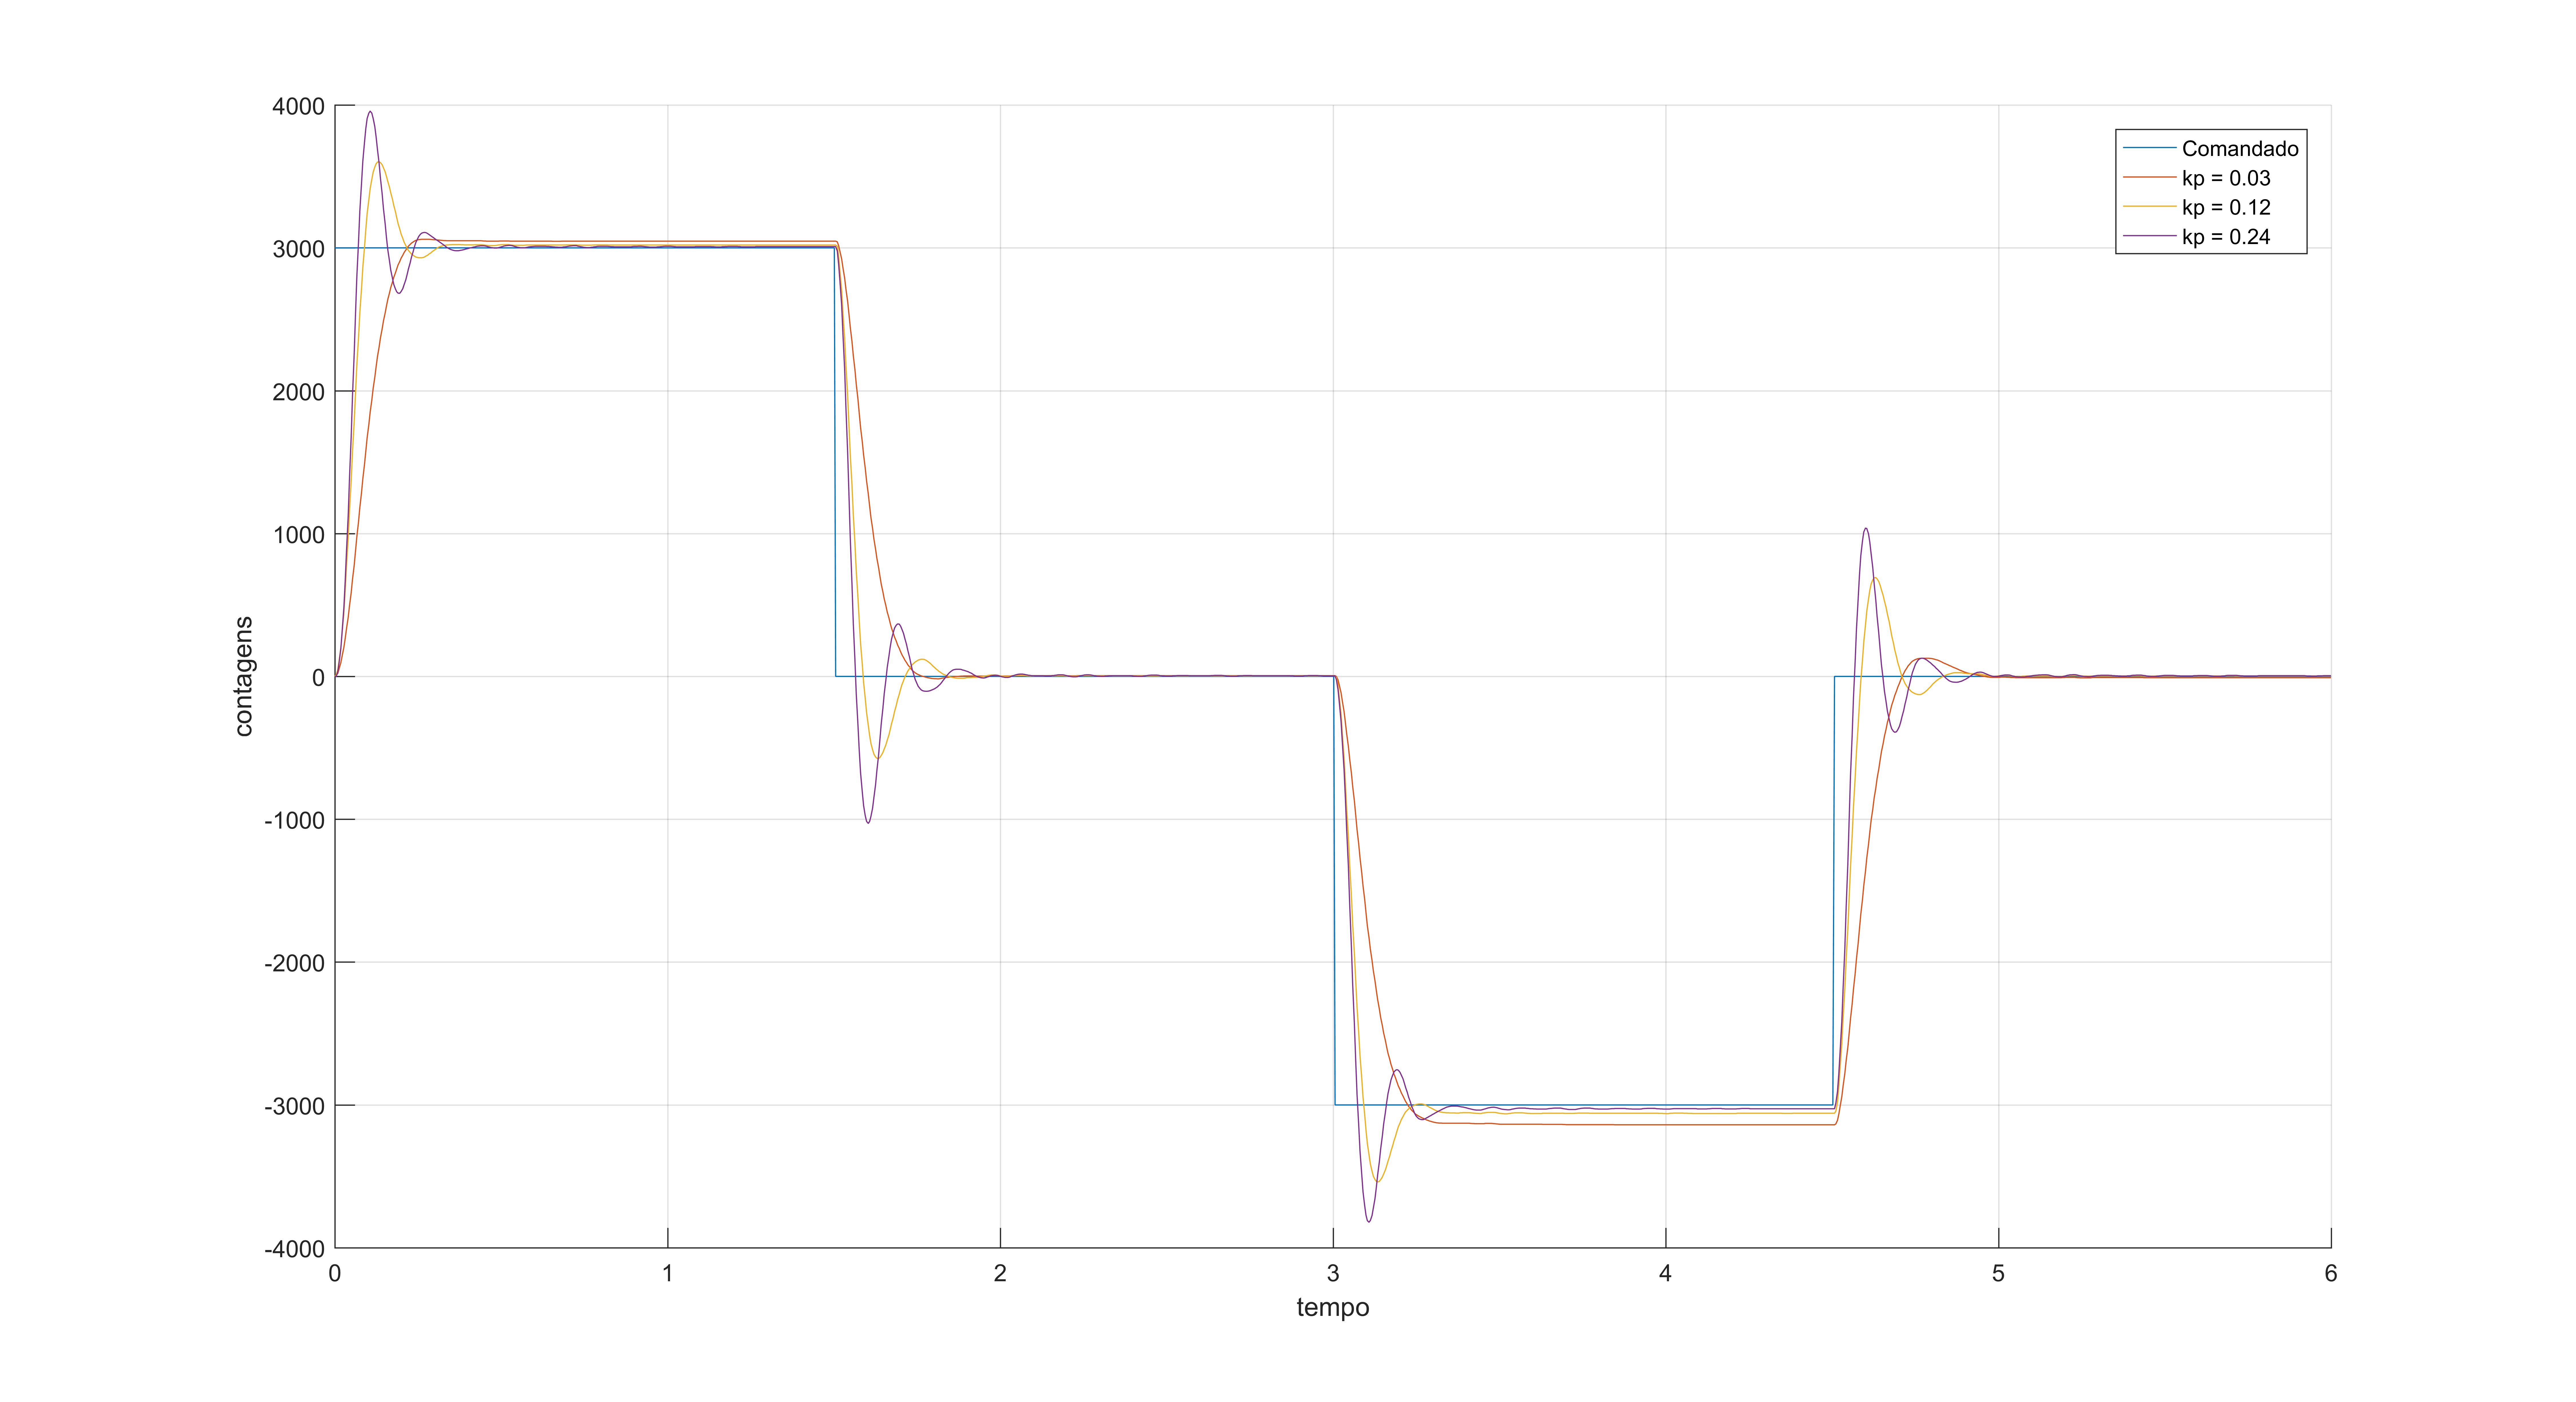
\includegraphics[width=\textwidth]{0_img/malha_fechada_corrigida.png}
    \caption{Saída do sistema em malha fechada com ganho $k_{pf}$ ajustado empiricamente para minimizar o erro em regime e diferentes valores de $k_p$}
    \label{fig:fechada_corrigida}
\end{figure}

\begin{figure}
    \centering
    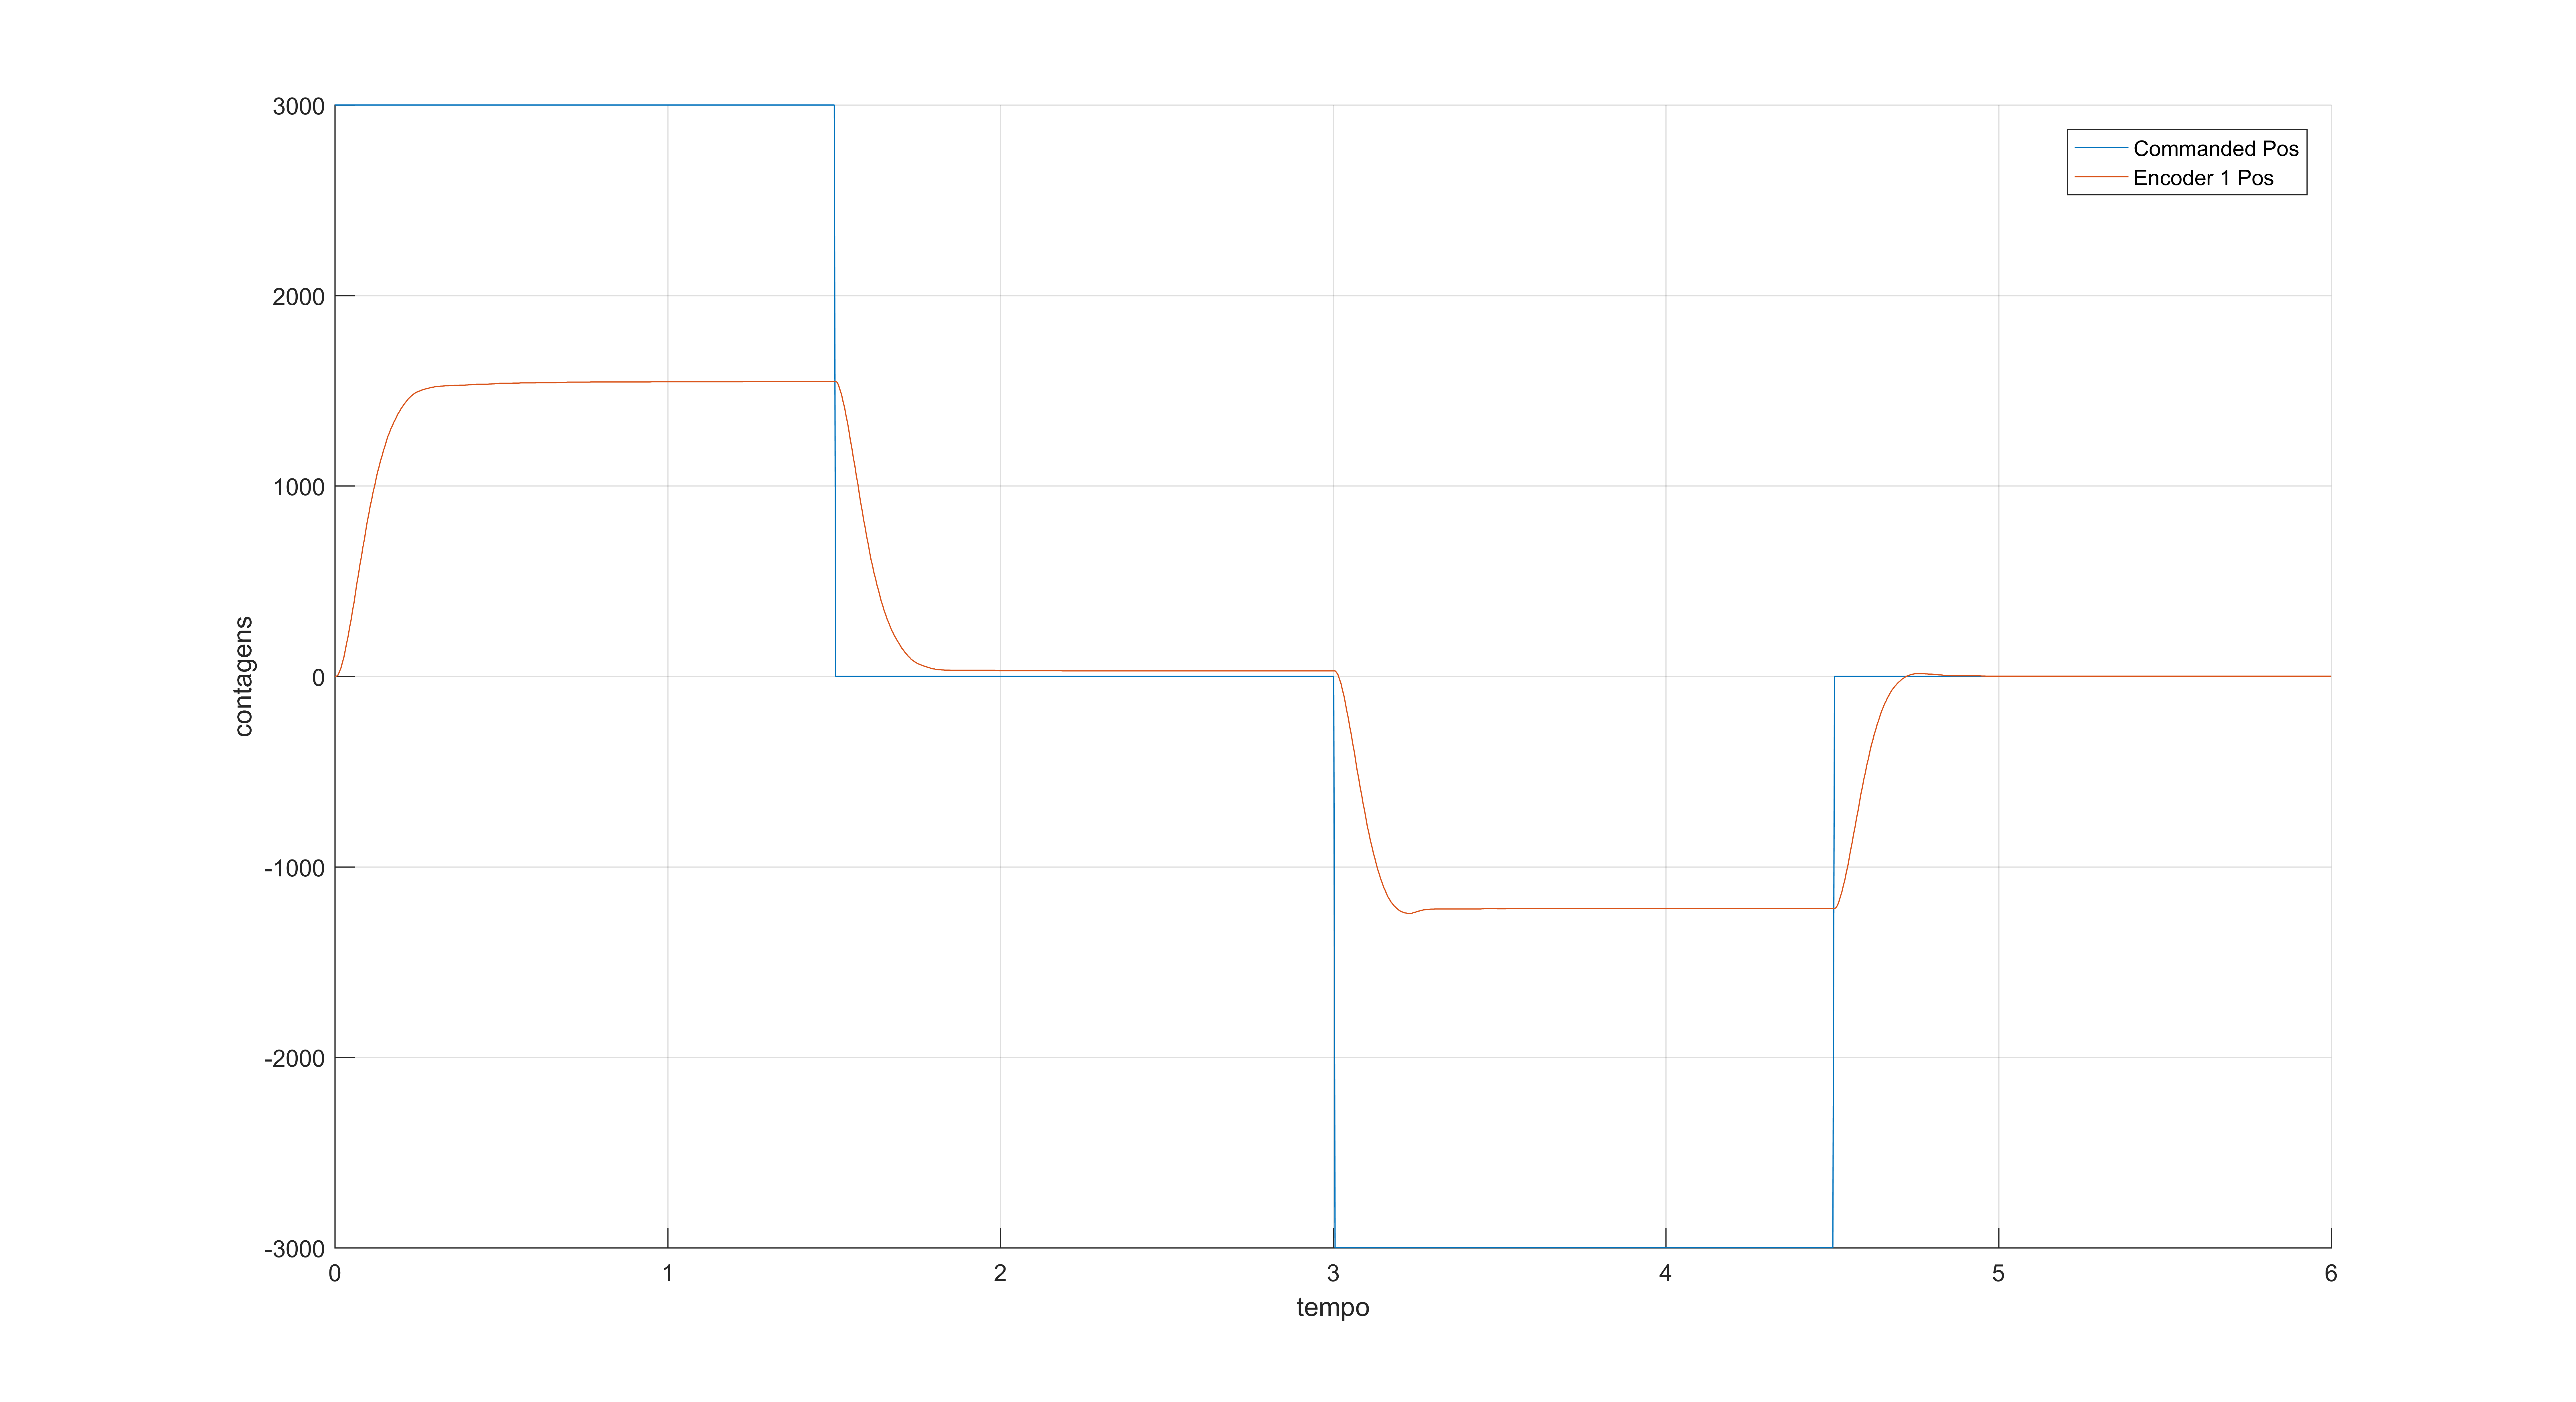
\includegraphics[width=\textwidth]{0_img/malha_aberta_mola.png}
    \caption{Saída do sistema em malha aberta com a mola trocada por uma de maior rigidez}
    \label{fig:aberta_mola}
\end{figure}

\begin{figure}
    \centering
    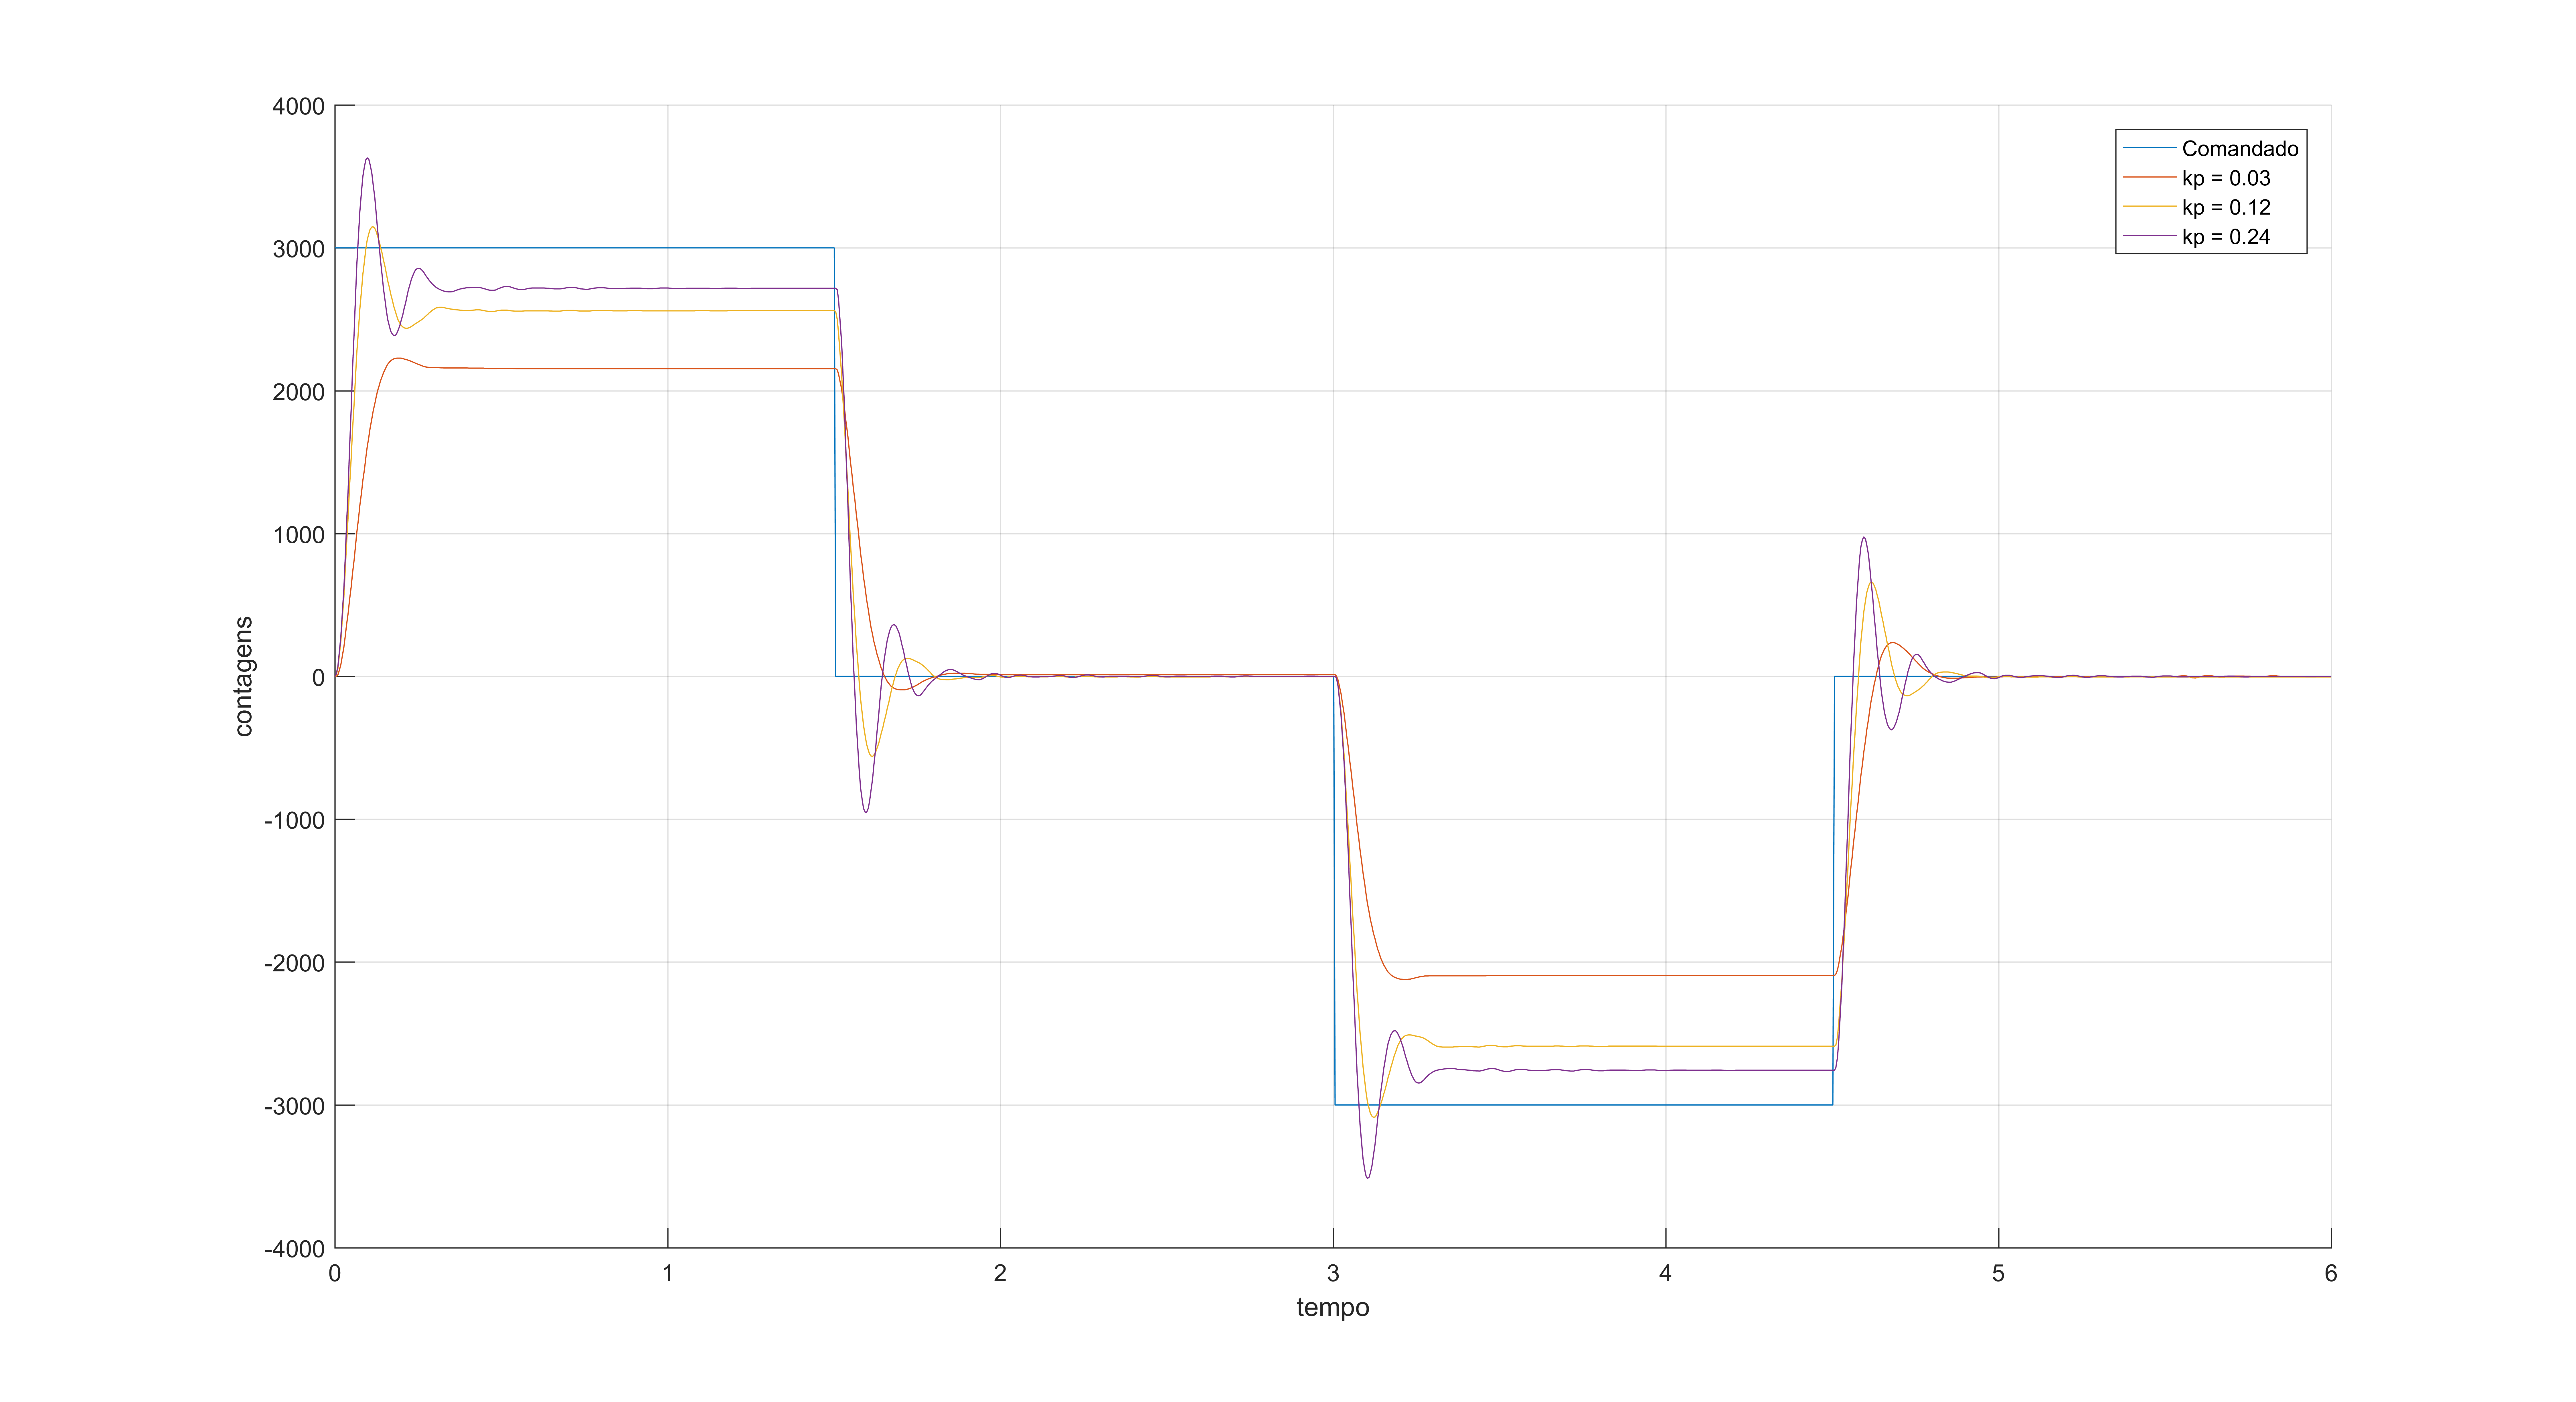
\includegraphics[width=\textwidth]{0_img/malha_fechada_mola.png}
    \caption{Saída do sistema em malha fechada com a mola trocada por uma de maior rigidez}
    \label{fig:fechada_mola}
\end{figure}

\end{document}